This section describes the software architecture of the \ac{KVS}. That includes
the operation principle in terms of transactions, storage, and concurrency as
well as the general structure.

\subsection{Two-Level Store}

As mentioned above, the \ac{KVS} resides entirely in main memory. This enables
fast access to all data within the database and makes swapping obsolete. In
return, the size of the database is bounded by the total \ac{NVRAM} capacity.
Apart from capacity, operating \ac{NVRAM} currently exhibits greater access
latencies compared to \ac{DRAM}. As pointed out in Chapter \ref{ch:nvram}, these
latencies mainly affect writes and are attributed to both technology parameters
and crash consistency measures. This work assumes, that even as technology
improves, crash consistency will continue to come a cost.

In an effort to mitigate these issues, the \ac{KVS} is designed to use volatile
\ac{RAM} in addition to \ac{NVRAM}. In order to achieve maximum performance, it
attempts to exploit the benefits of either technology while limiting the impact
of their drawbacks. For that purpose, the \ac{KVS} employs a two-level store
architecture as in \cite{bailey2013exploring}.

In a two-level store architecture, in-flight data from memory accesses may be
buffered in an intermediary storage medium. In this case, write operations are
buffered in volatile memory until their associated transaction commits. Only
when a transaction commits, all its updates are propagated to \ac{NVRAM}.
Otherwise, no user data is written to \ac{NVRAM}. Read operations are not
directly affected by the two-level store paradigm. In some cases, however, an
implementation may choose to buffer read operations, for instance to determine
serialization order.

The aim of the two-level store architecture is to reduce the impact of
\ac{NVRAM}-related latencies. Buffering updates to \ac{NVRAM} in volatile memory
has several advantages. First, updates are only posted to \ac{NVRAM} when they
need to be which can save both latency and memory bandwidth, especially when
aborts are frequent. Second, limiting updates to \ac{NVRAM} to commit phases
allows for bulk writes. This way, expensive consistency procedures do not have
to be performed repeatedly for a single transaction. Third, updated items in
volatile memory can be accessed with lower latencies, which is true for both
read and write operations. In the end, buffering updates also aids recovery, as
uncommitted data is guaranteed to be lost after a restart.

% \begin{figure}[!ht]
\begin{figure}
    \centering
    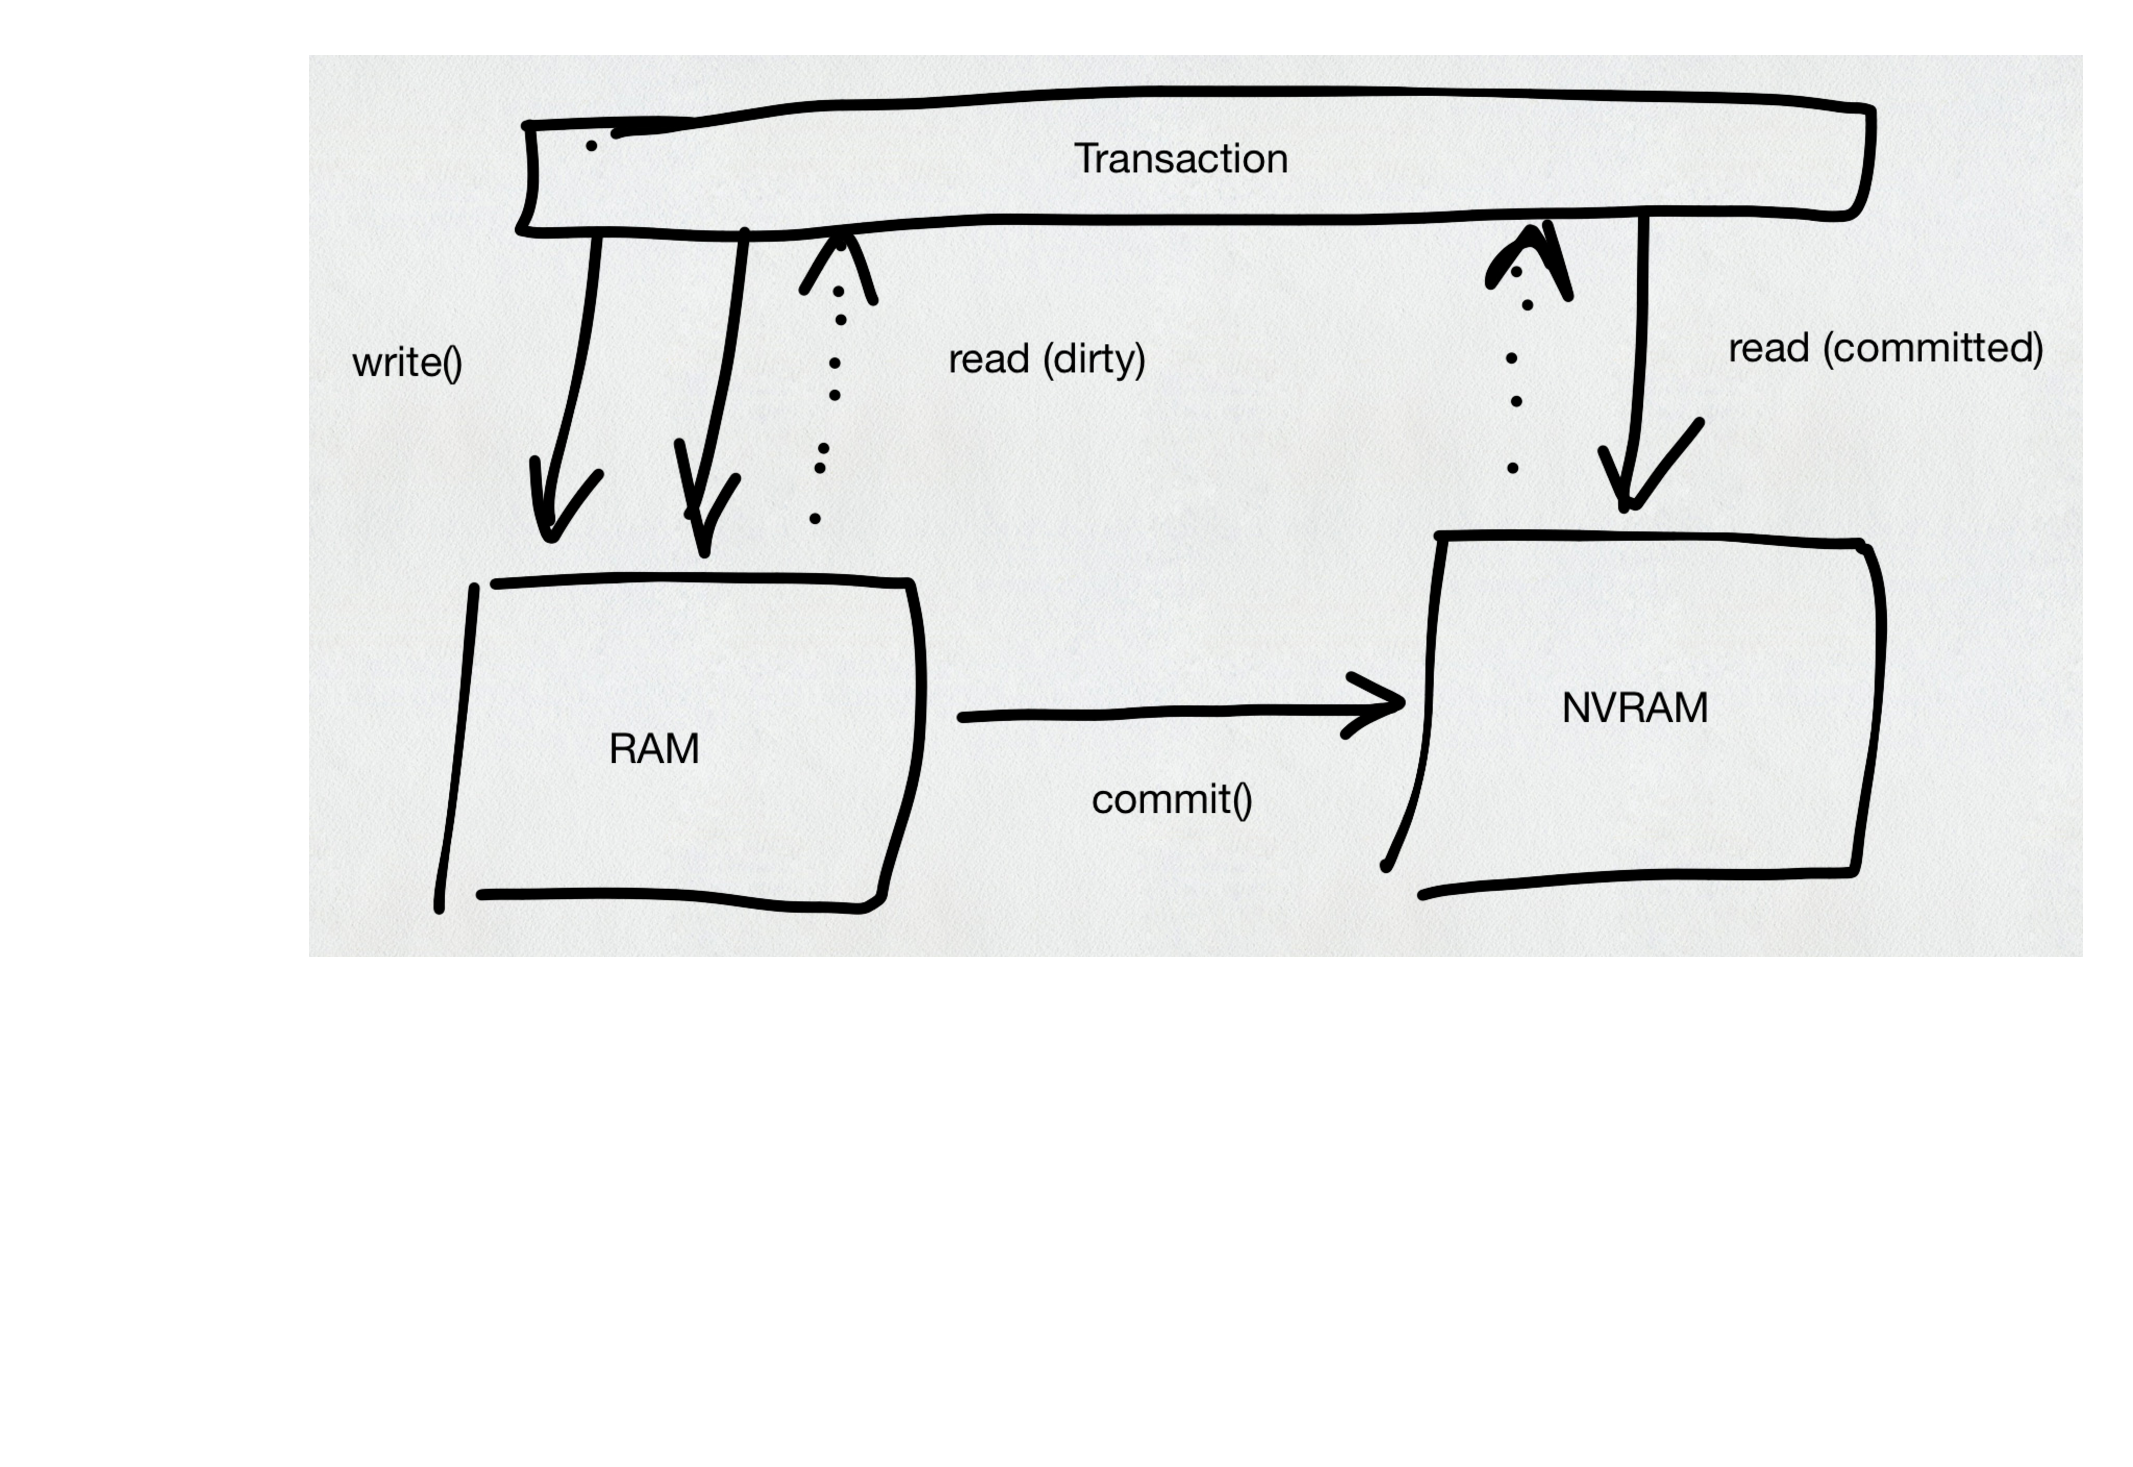
\includegraphics[width=\textwidth]{figures/drafts/concept-sys-two-level-store.pdf}
    \caption{}
    \label{fig:concept-two-level-store}
\end{figure}

\subsection{Transactions}

The \ac{KVS} supports full-featured and ACID-compliant transactions. Unlike
other works, this \ac{KVS} allows multiple operations to be enclosed in a single
transaction. The primary motivation behind this decision is to preserve
generality with regard to more complex \ac{DBMS}. Likewise, all transactions
must conform to the ACID properties to ensure data consistency. Nesting
transactions is not supported as use cases are too few to justify the additional
complexity.

Providing ACID support requires a conjunction of preventing erroneous behaviour
and restoring a previously sane state if an error occurs.

\paragraph{Isolation}

The cornerstone of this work is to ensure isolation between concurrent
transactions, that is concurrent transactions cannot observe each others
uncommitted actions. This is achieved with the two-level store architecture and
a serializing \ac{MVCC} protocol.

Each transaction is run in a separate thread. All modifications within a
transaction are buffered in thread-local volatile memory as opposed to updating
in-place. As a result, the database in \ac{NVRAM} does not reflect uncommitted
changes and can therefore not be used to observe such activity. Technically,
threads could spy on each others change buffers but such behaviour is neither
required nor intended.

Protecting transactions from observing concurrent updates, however, does not
imply transactionally consistent data. For this purpose, the \ac{KVS} employs a
serializing \ac{MVCC} protocol. When compared to locking-based approaches,
\ac{MVCC} protocols have shown better performance in read-intensive environments
and are used in many databases. In this case, the concrete protocol is a
serializing variant of \ac{SI} and serves two purposes: recovery and ensuring
all transactions behave as if run serially. On the one hand, timestamped
versions are used to keep track of modifications. On the other hand, a
copy-on-write mechanism is used to enable recoverable version histories without
logging.

\paragraph{Atomicity}

Atomicity means that a transactions either succeeds as a whole or it fails
entirely. This means that any traces of a failed transaction must be either
neutral or reverted. As with isolation, atomicity is achieved by the two-level
store architecture and the concurrency control protocol. The former ensures that
only modifications of committing transactions are written to durable memory.
That way, an incomplete or failed transaction cannot be globally observed. In
addition, the \ac{SI} protocol allows the system to always retrieve the latest
committed version of an item. Even if an update to \ac{NVRAM} fails, the
\ac{KVS} can always go back to the lastest committed version without performing
an actual rollback. However, in the event an update propagation to \ac{NVRAM} is
interrupted, partial write-backs may become durable. A typical scenario would be
a system crash or a power failure. In this case, the \ac{KVS} must ensure that
torn writes do not harm the consistency of data. Possible solutions for this
problem are recovery routines that locate and invalidate corrupted data or
designated bitfields that are guaranteed to be set only after the entire payload
has been written. The concrete recovery method to be used is
implementation-defined.

\paragraph{Durability \& Consistency}

Ensuring durability and consistency with \ac{NVRAM} requires special attention
and is covered in Chapter \ref{ch:concept-consistency}.

\subsection{Structures}

The \ac{KVS} resides entirely in main memory, that is, both volatile and
non-volatile memory. According to the two-level store architecture, the \ac{KVS}
is partitioned into two sections: a volatile and a non-volatile section.

\subsubsection{Volatile Section}

The volatile section only contains strictly volatile data, that is, losing these
data in a crash can never affect the durable part of the database. Most
importantly, that includes transaction control blocks and a transaction table.

\paragraph{Transaction Control Blocks}

From a software point of view, transactions can be modeled as a tuple of
attributes that describe the current state of a transactional context. Typical
attributes could be:

\begin{itemize}
    \item begin and end timestamps
    \item execution phase
    \item change sets
\end{itemize}

Throughout its lifetime, a transaction usually transitions through several
execution phases. Beginning with an \code{active} state once a transaction has
started, it may transition to \code{try\_commit} upon commit and finally
\code{committed} when it succeeds. Upon failure, a transaction could indicate a
\code{failed} state. The concrete set of phases is left to the implementation.

Change sets are required to buffer all modifications that a transaction carries
out. When a transaction commits all modifications are propagated to durable
memory. There may be several different change sets depending on the type of
operation, such as deleting or updating.

Transaction control blocks are volatile because, otherwise, incomplete
transactions would still have to be rolled back to satisfy atomicity.
Furthermore, preventing or removing partially committed change sets is handled
by recovery and \ac{NVRAM} management.

\paragraph{Transaction Table}

In order to manage currently running transactions, each new transaction is
placed inside a container. Especially with \ac{MVCC}, transactions may need a
way to inspect other transactions to detect conflicts. Since transactions run on
different threads or cores, respectively, the container is a globally shared
lookup table. In order to protect critical sections when accessing the table
locking or lock-free append-only approaches could be used. Completed
transactions may not be automatically removed from the table but collected by
garbage collector. The transaction table is volatile by implication as it only
contains transaction control blocks which are explicitly volatile.

% \begin{figure}[!ht]
\begin{figure}
    \centering
    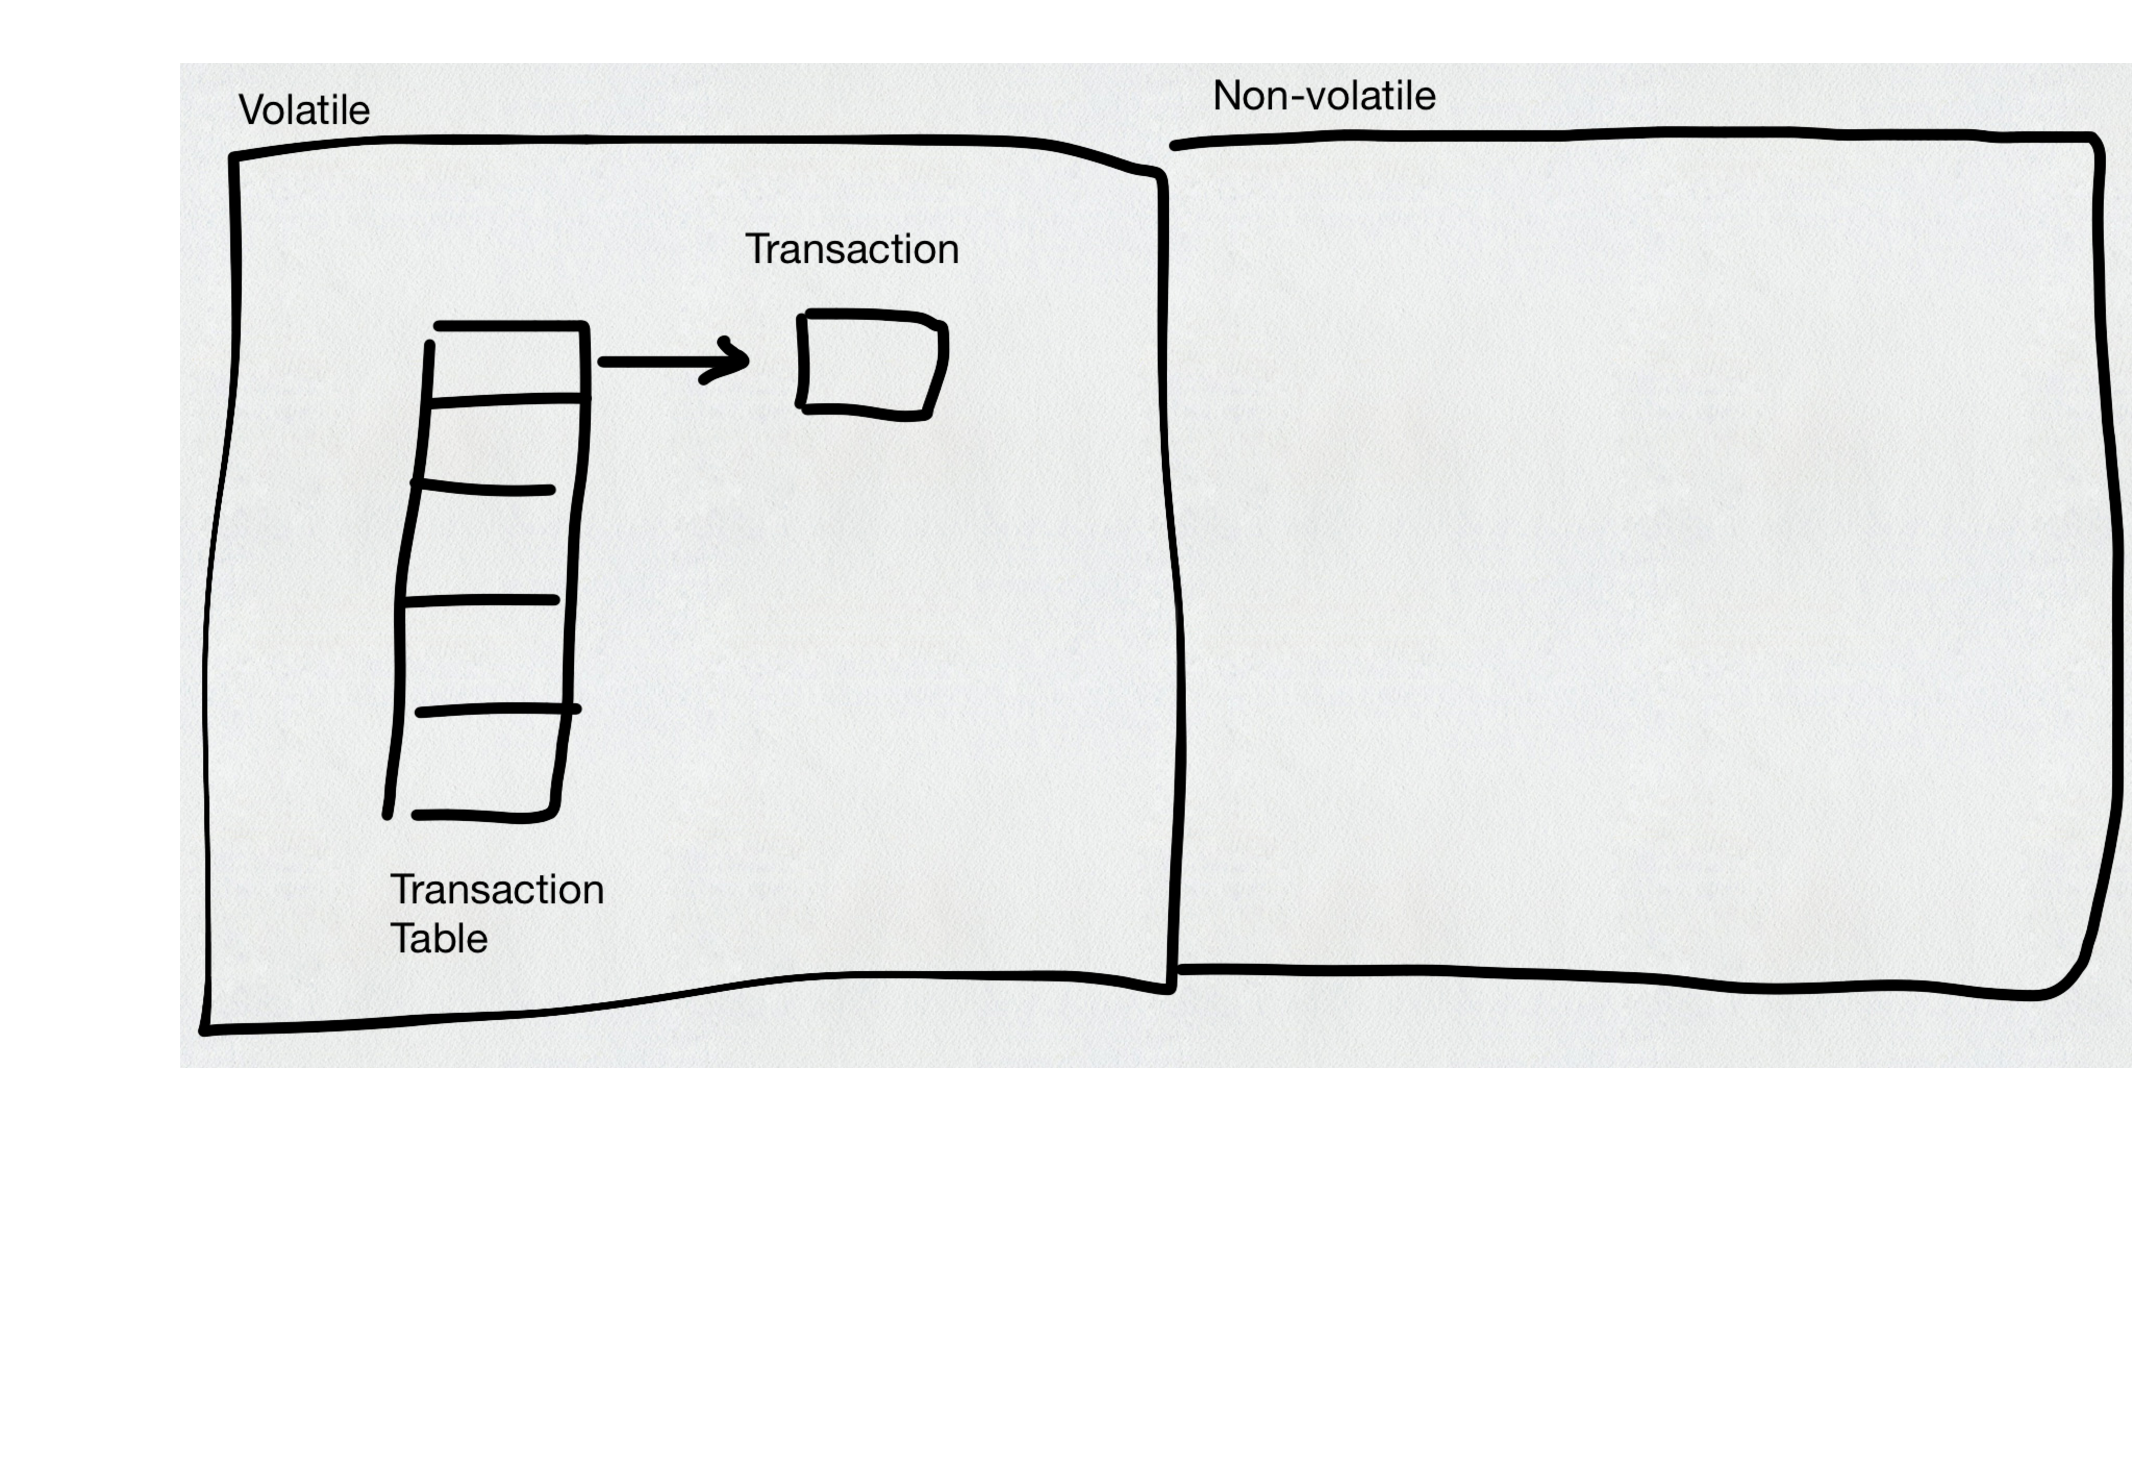
\includegraphics[width=\textwidth]{figures/drafts/concept-struct-volatile.pdf}
    \caption{}
    \label{fig:concept-struct-volatile}
\end{figure}

\subsubsection{Non-Volatile Section}

The non-volatile section stores all data that are durable across restarts. It
holds a control block, the index structure, and all data items mapped by the
index.

\paragraph{Control Block}

The control block is used to store a few essential metadata and for locating the
index after a restart. For that purpose, the control block is placed in a fixed
position of the \ac{KVS}' non-volatile region. Possible locations are the front
or rear end of the memory region. The index can be found by storing an offset or
pointer. Either way, the underlying system must provide a way to reuse or
recover a previous memory mapping, so both location methods are sufficient.

\paragraph{Index}

The index implements the actual \ac{KVS} paradigm by mapping keys to individual
data items. Note that, due to \ac{MVCC}, instead of mapping concrete data items,
each key maps to a history of versions of its associated item. It is the core
data structure of a \ac{KVS} and accessed by all transactions concurrently. As
such, the index is a strong contention point that is also very critical for the
performance of the \ac{KVS}. For that reason, selecting a suitable data
structure is crucial. The domain analysis in Chapter \ref{ch:kvs-nvram} shows
that many, if not most, \ac{KVS} rely on hash tables. Reasons are amortized
constant access, well-known array-like allocation schemes, and comparably low
complexity. B-trees or radix trees, on the other hand, are slower and optimized
for disk storage which was shown to be inappropriate for \ac{NVRAM}. Therefore,
this work opts for an index based on a hash table.

Operations on the index include adding, retrieving, and removing a key-value
pair. To prevent inconsistencies through race conditions, access must be
mutually exclusive. While locking can quickly become a bottleneck in
read-dominated scenarios, non-blocking data structures are generally slower and
more complex. The actual hashing method is an implementation detail.

\paragraph{Histories}

The index maps each key to a chain of versions of a data item. Before an
operation on an item can begin, the \ac{MVCC} algorithm has to determine which
version of the item is visible to the requesting transaction. As a result,
histories may be iterated frequently. Also multiple transactions may access the
same history at a time, so there may be overlapping accesses. However,
transactions never remove and only add new versions at the back of the history.
Therefore, contention may be high but mostly read-only. In order to account for
these characteristics, an array-like data structure may be the most appropriate
choice as opposed to a list. Consecutive access in arrays is less likely to
cause page faults and can benefit from hardware prefetching. Also arrays have
simpler allocation patterns compared to lists. Problems arise with garbage
collection which could perform random-access modifications to the history. Since
garbage collection would break the scope of this work, it is assumed to be
absent or as non-invasive as possible.

% \begin{figure}[!ht]
\begin{figure}
    \centering
    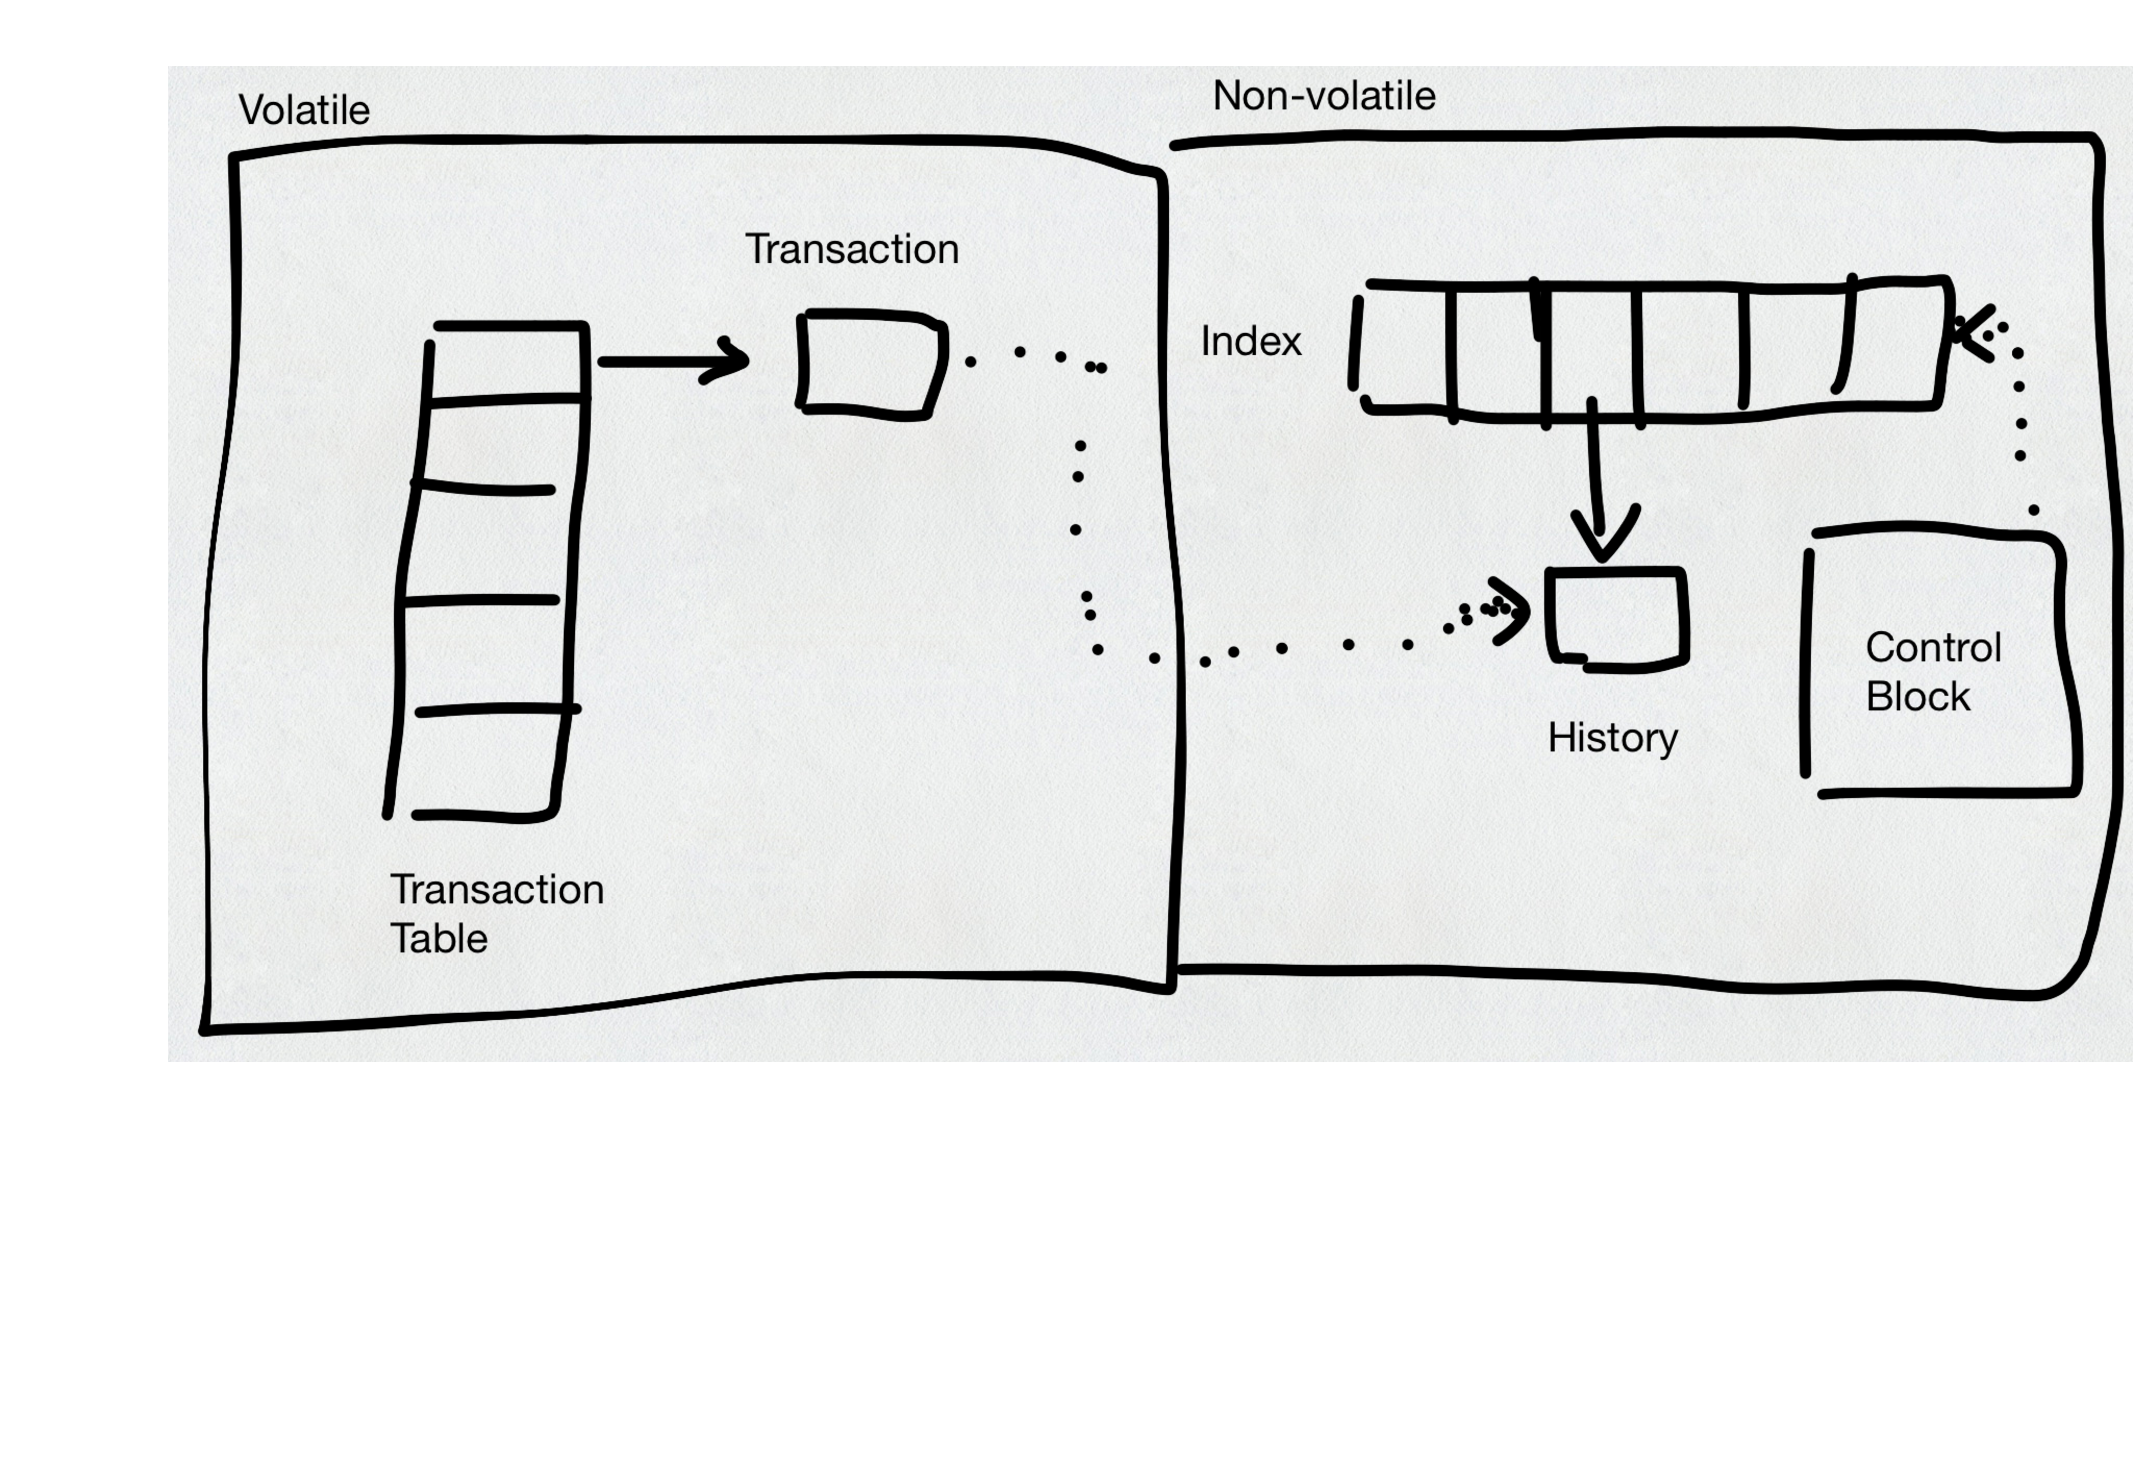
\includegraphics[width=\textwidth]{figures/drafts/concept-struct-complete.pdf}
    \caption{}
    \label{fig:concept-struct-complete}
\end{figure}
